\section{Encoder-Decoder Architectures}

\begin{frame}
	\frametitle{Encoder-Decoder Architectures for Modelling Sequences}

	Alternative to RNNs and CNNs are \alert{encoder-decoder} class of
	architectures

	\begin{center}
		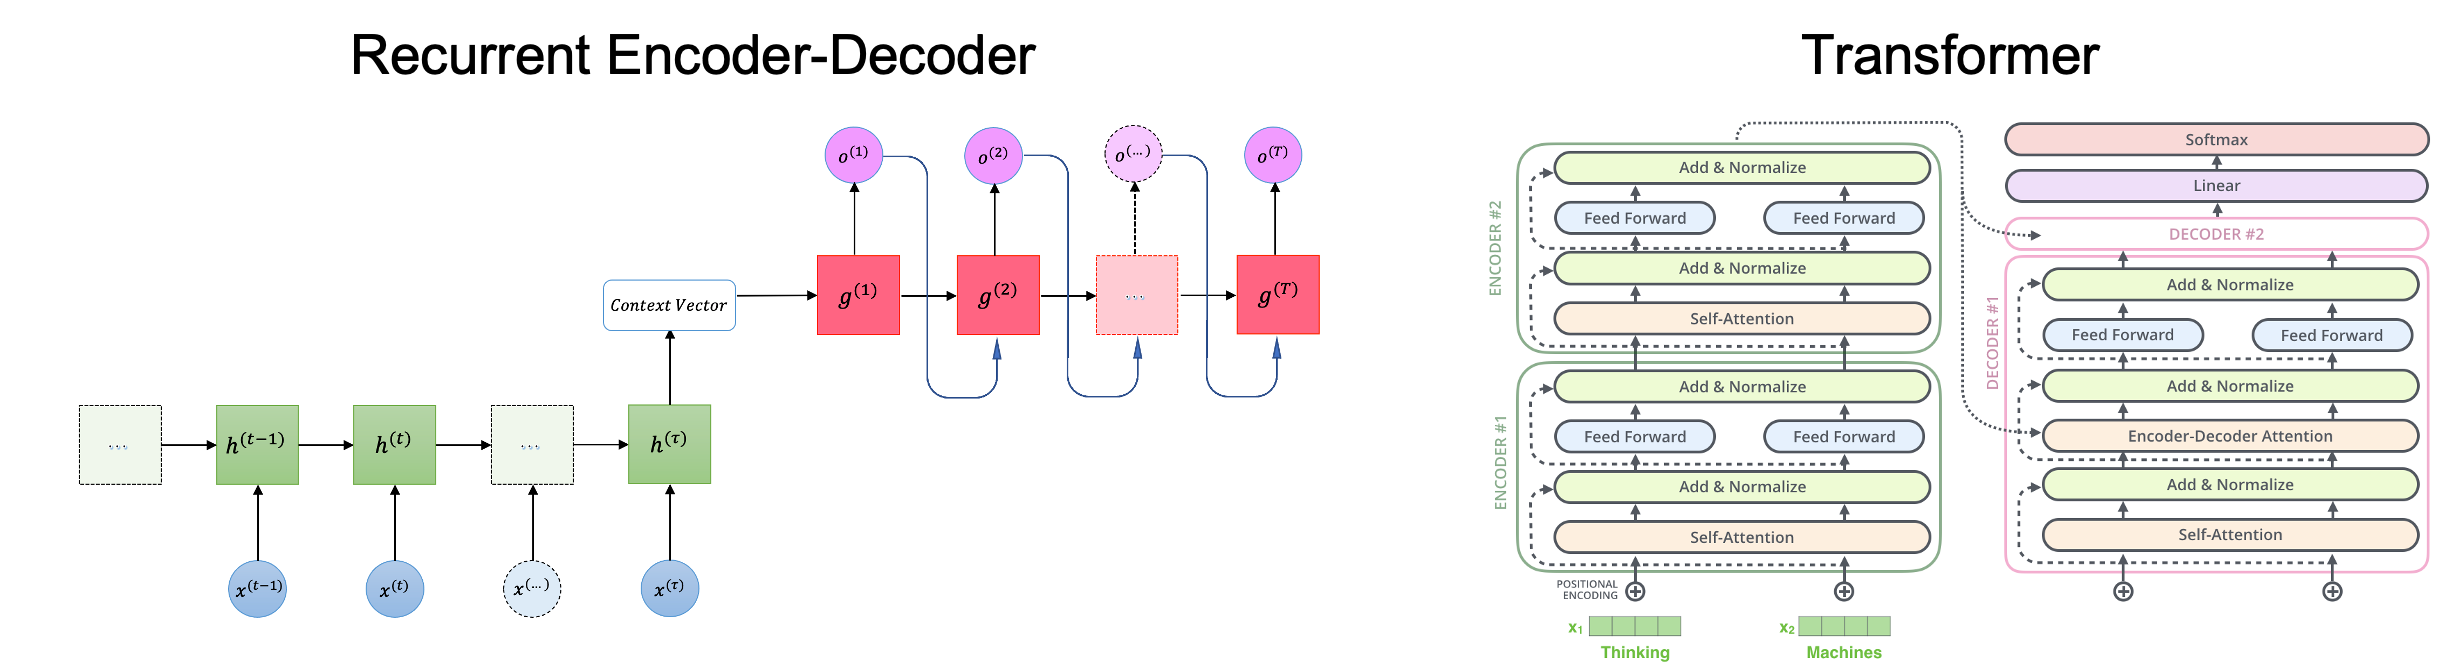
\includegraphics[width=\textwidth]{figures/ed_transf.png}
	\end{center}


    \begin{empheq}[box=\mymath]{gather*}
        \text{
			How do they compare with RNN and CNN?
        }
    \end{empheq}

\end{frame}

\begin{frame}
	\frametitle{Linear Recurrent Encoder-Decoder}

	\begin{center}
		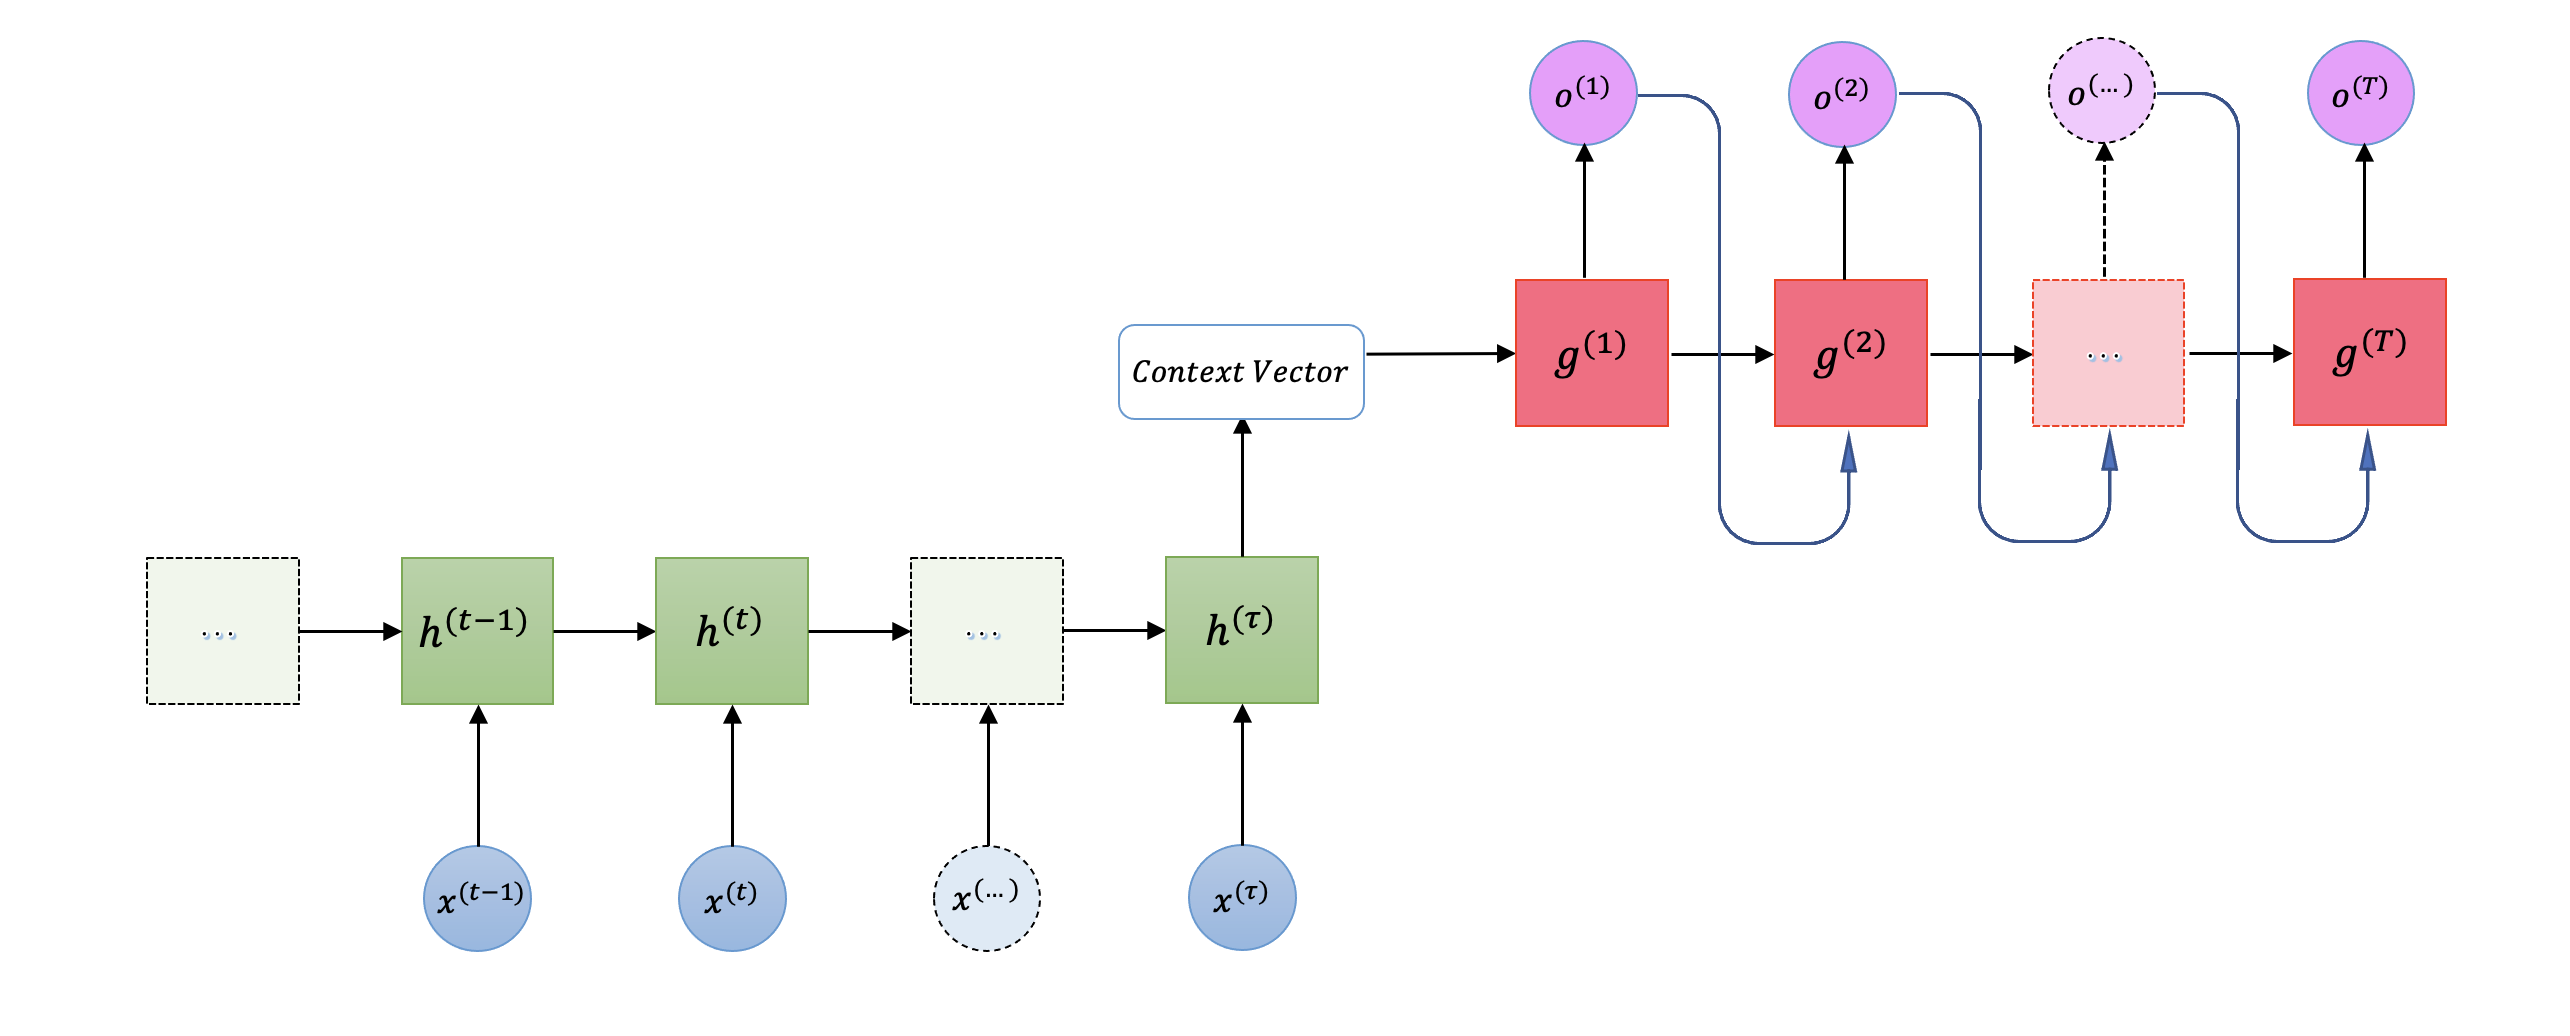
\includegraphics[width=0.8\textwidth]{figures/encdec.png}
	\end{center}

	As before, linear continuous variant gives the following dynamics
	\begin{equation*}
		\begin{matrix}
			\dot{h}_s = Wh_s+Ux_s,
			& v=Qh_0,
			& s\leq 0,
			& h_s \in \R^{m_E}, v \in \R^{N}\\
			\dot{g}_t = Vg_t,
			& g_0=Pv,
			&
			& g_t \in \R^{m_D}
			\\
			y_t = c^\top g_t,
			&
			& t\ge 0
			&
		\end{matrix}
	\end{equation*}
	% \begin{equation*}
	% 	\begin{aligned}
	% 		\dot{h}_s
	% 		& = Wh_s+Ux_s,
	% 		&& v=Qh_0, \quad &s\leq 0,
	% 		&&h_s \in \R^{m_E},
	% 		v \in \R^{N}
	% 		\\
	% 		\dot{g}_t
	% 		& = Vg_t,
	% 		&& g_0=Pv,
	% 		&& g_t \in \R^{m_D}
	% 		\\
	% 		y_t
	% 		&=c^\top g_t,
	% 		&&
	% 		&&t\ge 0,
	% 		% &V\in\mathbb R^{m_D\times m_D}, U\in\mathbb R^{m_E\times d},\\
	% 		% Q\in\mathbb R^{N\times m_E}, & P\in\mathbb R^{m_D\times N}.
	% 	\end{aligned}
	% \end{equation*}

\end{frame}

\begin{frame}
	\frametitle{Linear Recurrent Encoder-Decoder Hypothesis Space}

	The hypothesis space is
	\begin{equation*}
		\henc^{(m_E,m_D,N)} :=
		\Big\{\bhh: \hat H_t = \int_{0}^{\infty} c^\top e^{Vt} PQe^{W s} U x_{t-s} ds \Big\}
	\end{equation*}
	and
	\begin{equation*}
		\henc := \bigcup_{N,m_E,m_D \in \mathbb{N}_+}
		\henc^{(m_E,m_D,N)}
	\end{equation*}

	\pause{}

	\medskip
	\medskip

	\begin{empheq}[box=\mymath]{gather*}
		\text{
			How is this different from RNN/CNN?
		}
    \end{empheq}

\end{frame}

\begin{frame}
	\frametitle{Approximation Guarantee (Density)}

	\begin{alertblock}{Theorem [LJL, 2022]}
		Let $\{ \Htar_t : t\in\R \}$ be a family of continuous,
		linear, \sout{causal}, regular and \sout{time-homogeneous} functionals
		on $C_0(\R,\R^d)$.
		Then, for any $\epsilon > 0$ there exists $\{ \wh{H}_t : t\in \R \} \in \henc$ such that
		\begin{equation*}
			\| \bm \Htar - \wh{\bm H} \|
			% \sup_{t\in\R}
			% \| \Htar_t - \wh{H}_t \|
			\equiv
			\sup_{t\in\R}
			\sup_{\| \*x \|_C \leq 1}
			|
			\Htar_t(\*x) - \wh{H}_t(\*x)
			|
			\leq \epsilon.
		\end{equation*}
	\end{alertblock}

	Main idea: Riesz representation for non-time-homogeneous functional
	\begin{equation*}
		H^*_t(\*x) =
		\int_{0}^{\infty}
		x_{t-s}^\tp \rho(t,s) ds
	\end{equation*}
	Then, recurrent encoder-decoder approximates $\rho(t,s)$ by
	$c^\top e^{Vt} PQe^{W s} U$


	\blfootnote{
		\fullcite{li2021approxed}
	}
\end{frame}

\begin{frame}
	\frametitle{The Temporal Product Structure}

	Notice that recurrent encoder-decoder approximates
	\begin{equation*}
		\rho^{(\bm H^*)}(t,s)
		\qquad
		\rightarrow
		\qquad
		\underbrace{
			c^\top e^{Vt}P
		}_{
			{\bm \phi}(t)
		}
		\cdot
		\underbrace{
			Qe^{W s} U
		}_{
			{\bm \psi}(s)
		}
		=
		\sum_{n=1}^{N}
		\phi_n(t) \psi_n(s)
	\end{equation*}
	\begin{itemize}[<+->]
		\item
		Hence, $N$ can be taken small if ${\bm \rho}^{\bm H^*}$
		is of a \alert{temporal product structure}, i.e.
		having low effective rank under functional SVD
		(Proper Orthogonal Decomposition, POD)!
		\item
		This leads to precise approximation rates in terms of
		$\{m_E, m_D,N\}$ \refhl{[LJL, 2022]}
	\end{itemize}


	\blfootnote{
		\fullcite{li2021approxed}
	}
\end{frame}

\begin{frame}
	\frametitle{Low vs High (Effective) Rank Relationships}

	\begin{center}
		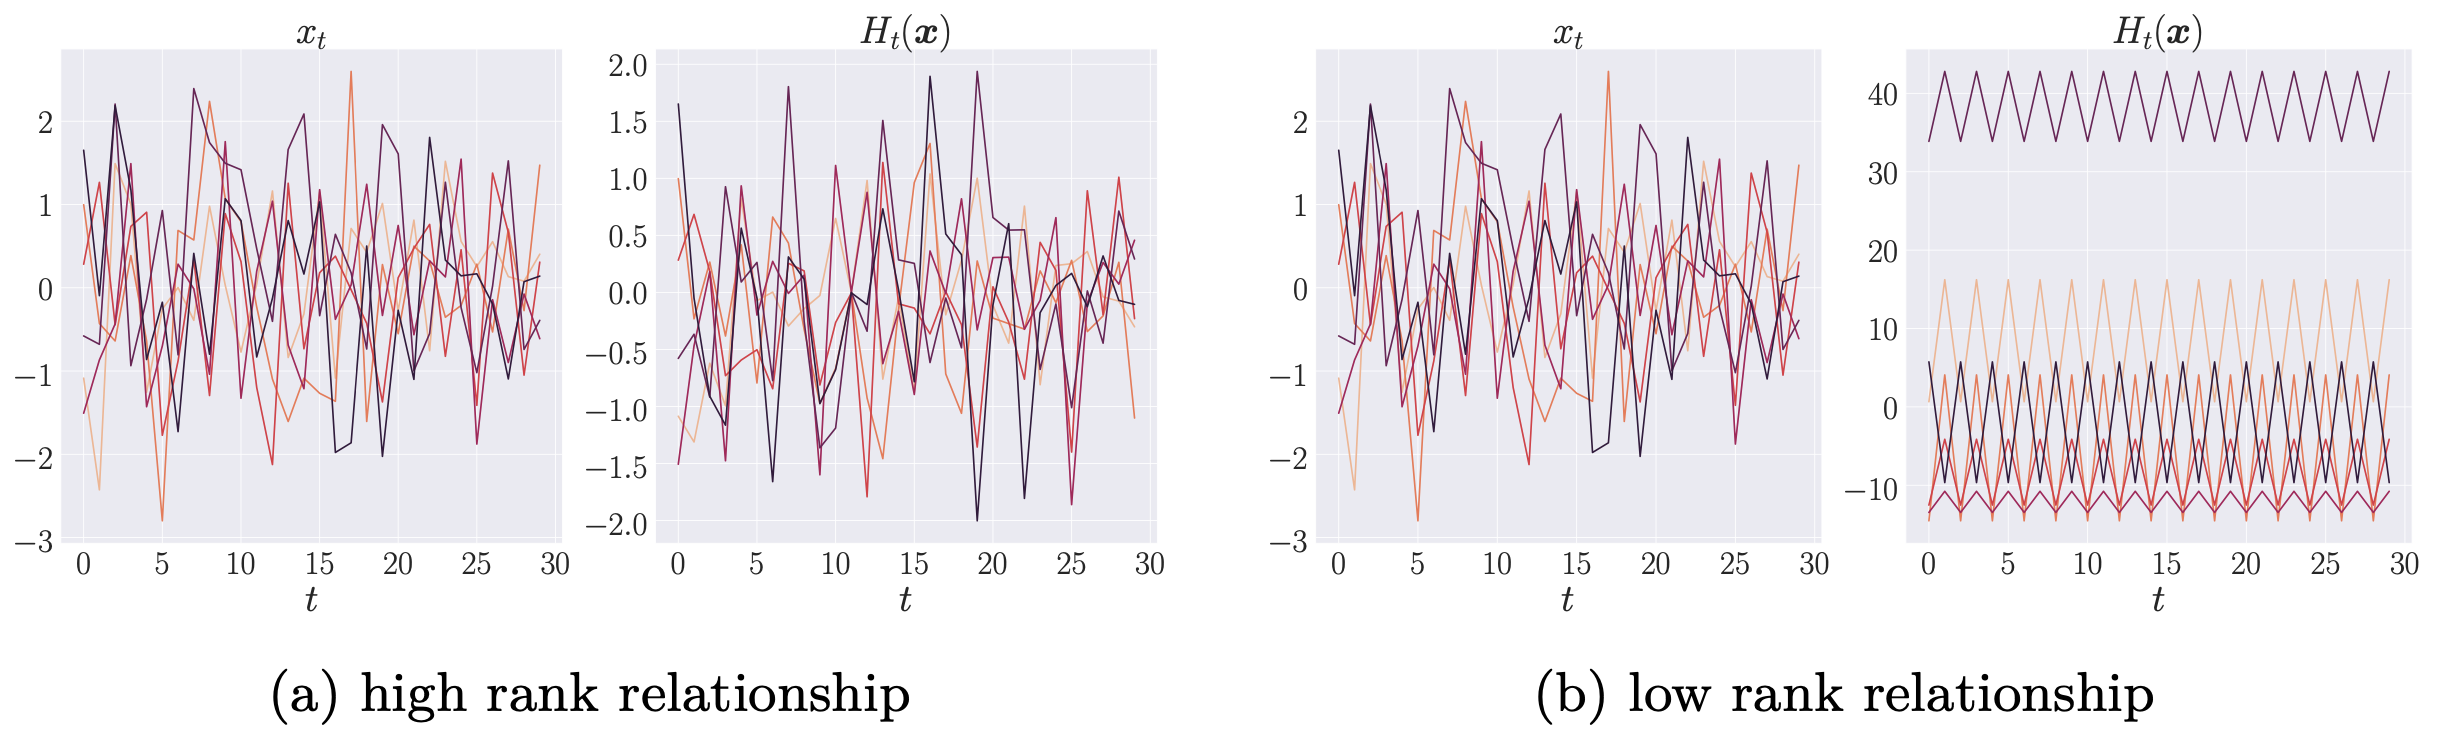
\includegraphics[width=\textwidth]{figures/low_high_rank.png}
	\end{center}

	\begin{empheq}[box=\mymath]{equation*}
		\textbf{Insight:}
		\qquad
		\begin{aligned}
			&\text{
				Encoder-decoders are most effective in capturing
			}\\
			&\text{
				temporal product structures with low effective rank!
			}
		\end{aligned}
    \end{empheq}

\end{frame}
